%  LaTeX support: latex@mdpi.com 
%  For support, please attach all files needed for compiling as well as the log file, and specify your operating system, LaTeX version, and LaTeX editor.

%=================================================================
\documentclass[journal]{Definitions/mdpi} 

%--------------------
% Class Options:
%--------------------
%----------
% journal
%----------
% Choose between the following MDPI journals:
% acoustics, actuators, addictions, admsci, adolescents, aerobiology, aerospace, agriculture, agriengineering, agrochemicals, agronomy, ai, air, algorithms, allergies, alloys, analytica, analytics, anatomia, animals, antibiotics, antibodies, antioxidants, applbiosci, appliedchem, appliedmath, applmech, applmicrobiol, applnano, applsci, aquacj, architecture, arm, arthropoda, arts, asc, asi, astronomy, atmosphere, atoms, audiolres, automation, axioms, bacteria, batteries, bdcc, behavsci, beverages, biochem, bioengineering, biologics, biology, biomass, biomechanics, biomed, biomedicines, biomedinformatics, biomimetics, biomolecules, biophysica, biosensors, biotech, birds, bloods, blsf, brainsci, breath, buildings, businesses, cancers, carbon, cardiogenetics, catalysts, cells, ceramics, challenges, chemengineering, chemistry, chemosensors, chemproc, children, chips, cimb, civileng, cleantechnol, climate, clinpract, clockssleep, cmd, coasts, coatings, colloids, colorants, commodities, compounds, computation, computers, condensedmatter, conservation, constrmater, cosmetics, covid, crops, cryptography, crystals, csmf, ctn, curroncol, cyber, dairy, data, ddc, dentistry, dermato, dermatopathology, designs, devices, diabetology, diagnostics, dietetics, digital, disabilities, diseases, diversity, dna, drones, dynamics, earth, ebj, ecologies, econometrics, economies, education, ejihpe, electricity, electrochem, electronicmat, electronics, encyclopedia, endocrines, energies, eng, engproc, entomology, entropy, environments, environsciproc, epidemiologia, epigenomes, est, fermentation, fibers, fintech, fire, fishes, fluids, foods, forecasting, forensicsci, forests, foundations, fractalfract, fuels, future, futureinternet, futurepharmacol, futurephys, futuretransp, galaxies, games, gases, gastroent, gastrointestdisord, gels, genealogy, genes, geographies, geohazards, geomatics, geosciences, geotechnics, geriatrics, grasses, gucdd, hazardousmatters, healthcare, hearts, hemato, hematolrep, heritage, higheredu, highthroughput, histories, horticulturae, hospitals, humanities, humans, hydrobiology, hydrogen, hydrology, hygiene, idr, ijerph, ijfs, ijgi, ijms, ijns, ijpb, ijtm, ijtpp, ime, immuno, informatics, information, infrastructures, inorganics, insects, instruments, inventions, iot, j, jal, jcdd, jcm, jcp, jcs, jcto, jdb, jeta, jfb, jfmk, jimaging, jintelligence, jlpea, jmmp, jmp, jmse, jne, jnt, jof, joitmc, jor, journalmedia, jox, jpm, jrfm, jsan, jtaer, jvd, jzbg, kidneydial, kinasesphosphatases, knowledge, land, languages, laws, life, liquids, literature, livers, logics, logistics, lubricants, lymphatics, machines, macromol, magnetism, magnetochemistry, make, marinedrugs, materials, materproc, mathematics, mca, measurements, medicina, medicines, medsci, membranes, merits, metabolites, metals, meteorology, methane, metrology, micro, microarrays, microbiolres, micromachines, microorganisms, microplastics, minerals, mining, modelling, molbank, molecules, mps, msf, mti, muscles, nanoenergyadv, nanomanufacturing,\gdef\@continuouspages{yes}} nanomaterials, ncrna, ndt, network, neuroglia, neurolint, neurosci, nitrogen, notspecified, %%nri, nursrep, nutraceuticals, nutrients, obesities, oceans, ohbm, onco, %oncopathology, optics, oral, organics, organoids, osteology, oxygen, parasites, parasitologia, particles, pathogens, pathophysiology, pediatrrep, pharmaceuticals, pharmaceutics, pharmacoepidemiology,\gdef\@ISSN{2813-0618}\gdef\@continuous pharmacy, philosophies, photochem, photonics, phycology, physchem, physics, physiologia, plants, plasma, platforms, pollutants, polymers, polysaccharides, poultry, powders, preprints, proceedings, processes, prosthesis, proteomes, psf, psych, psychiatryint, psychoactives, publications, quantumrep, quaternary, qubs, radiation, reactions, receptors, recycling, regeneration, religions, remotesensing, reports, reprodmed, resources, rheumato, risks, robotics, ruminants, safety, sci, scipharm, sclerosis, seeds, sensors, separations, sexes, signals, sinusitis, skins, smartcities, sna, societies, socsci, software, soilsystems, solar, solids, spectroscj, sports, standards, stats, std, stresses, surfaces, surgeries, suschem, sustainability, symmetry, synbio, systems, targets, taxonomy, technologies, telecom, test, textiles, thalassrep, thermo, tomography, tourismhosp, toxics, toxins, transplantology, transportation, traumacare, traumas, tropicalmed, universe, urbansci, uro, vaccines, vehicles, venereology, vetsci, vibration, virtualworlds, viruses, vision, waste, water, wem, wevj, wind, women, world, youth, zoonoticdis 
% For posting an early version of this manuscript as a preprint, you may use "preprints" as the journal. Changing "submit" to "accept" before posting will remove line numbers.

%---------
% article
%---------
% The default type of manuscript is "article", but can be replaced by: 
% abstract, addendum, article, book, bookreview, briefreport, casereport, comment, commentary, communication, conferenceproceedings, correction, conferencereport, entry, expressionofconcern, extendedabstract, datadescriptor, editorial, essay, erratum, hypothesis, interestingimage, obituary, opinion, projectreport, reply, retraction, review, perspective, protocol, shortnote, studyprotocol, systematicreview, supfile, technicalnote, viewpoint, guidelines, registeredreport, tutorial
% supfile = supplementary materials

%----------
% submit
%----------
% The class option "submit" will be changed to "accept" by the Editorial Office when the paper is accepted. This will only make changes to the frontpage (e.g., the logo of the journal will get visible), the headings, and the copyright information. Also, line numbering will be removed. Journal info and pagination for accepted papers will also be assigned by the Editorial Office.

%------------------
% moreauthors
%------------------
% If there is only one author the class option oneauthor should be used. Otherwise use the class option moreauthors.

%---------
% pdftex
%---------
% The option pdftex is for use with pdfLaTeX. Remove "pdftex" for (1) compiling with LaTeX & dvi2pdf (if eps figures are used) or for (2) compiling with XeLaTeX.

%=================================================================
% MDPI internal commands - do not modify
\firstpage{1} 
\makeatletter 
\setcounter{page}{\@firstpage} 
\makeatother
\pubvolume{1}
\issuenum{1}
\articlenumber{0}
\pubyear{2024}
\copyrightyear{2024}
%\externaleditor{Academic Editor: Firstname Lastname}
\datereceived{ } 
\daterevised{ } % Comment out if no revised date
\dateaccepted{ } 
\datepublished{ } 
%\datecorrected{} % For corrected papers: "Corrected: XXX" date in the original paper.
%\dateretracted{} % For corrected papers: "Retracted: XXX" date in the original paper.
\hreflink{https://doi.org/} % If needed use \linebreak
%\doinum{}
%\pdfoutput=1 % Uncommented for upload to arXiv.org
%\CorrStatement{yes}  % For updates


%=================================================================
% Add packages and commands here. The following packages are loaded in our class file: fontenc, inputenc, calc, indentfirst, fancyhdr, graphicx, epstopdf, lastpage, ifthen, float, amsmath, amssymb, lineno, setspace, enumitem, mathpazo, booktabs, titlesec, etoolbox, tabto, xcolor, colortbl, soul, multirow, microtype, tikz, totcount, changepage, attrib, upgreek, array, tabularx, pbox, ragged2e, tocloft, marginnote, marginfix, enotez, amsthm, natbib, hyperref, cleveref, scrextend, url, geometry, newfloat, caption, draftwatermark, seqsplit
% cleveref: load \crefname definitions after \begin{document}

%=================================================================
% Please use the following mathematics environments: Theorem, Lemma, Corollary, Proposition, Characterization, Property, Problem, Example, ExamplesandDefinitions, Hypothesis, Remark, Definition, Notation, Assumption
%% For proofs, please use the proof environment (the amsthm package is loaded by the MDPI class).

%=================================================================
% Full title of the paper (Capitalized)
\Title{Enhanced Security Protocols for IoT-Based Precision Agriculture: A Comparative Analysis of Lightweight Cryptography Solutions}

% MDPI internal command: Title for citation in the left column
\TitleCitation{Title}

% Author Orchid ID: enter ID or remove command
\newcommand{\orcidauthorA}{0000-0000-0000-000X} % Add \orcidA{} behind the author's name
%\newcommand{\orcidauthorB}{0000-0000-0000-000X} % Add \orcidB{} behind the author's name

% Authors, for the paper (add full first names)
\Author{Saraswathi Gurram $^{1,\dagger,\ddagger}$\orcidA{}, Nagender Kumar.S $^{2,\ddagger}$ }

%\longauthorlist{yes}

% MDPI internal command: Authors, for metadata in PDF
\AuthorNames{Saraswathi Gurram,Nagender Kumar}

% MDPI internal command: Authors, for citation in the left column
\AuthorCitation{Saraswathi Gurram, Nagender Kumar .s }
% If this is a Chicago style journal: Lastname, Firstname, Firstname Lastname, and Firstname Lastname.

% Affiliations / Addresses (Add [1] after \address if there is only one affiliation.)
\address{%
$^{1}$ \quad Affiliation 1; 22mcpc16@uohyd.ac.in\\
$^{2}$ \quad Affiliation 2; nks@uohyd.ac.in }

% Contact information of the corresponding author
\corres{Correspondence: e-mail@e-mail.com; Tel.: (optional; include country code; if there are multiple corresponding authors, add author initials) +xx-xxxx-xxx-xxxx (F.L.)}

% Current address and/or shared authorship
\firstnote{University of Hyderabad : Affiliation.}  % Current address should not be the same as any items in the Affiliation section.
\secondnote{These authors contributed equally to this work.}
% The commands \thirdnote{} till \eighthnote{} are available for further notes

%\simplesumm{} % Simple summary

%\conference{} % An extended version of a conference paper

% Abstract (Do not insert blank lines, i.e. \\) 
\abstract{Securing data transmission in IoT-based precision agriculture systems is critical due to the vulnerabilities of resource-constrained devices and the sensitivity of environmental data \cite{ref-journal2, ref-journal5}. This study introduces a lightweight RC4 encryption-based framework to achieve end-to-end security for smart irrigation systems. Environmental data, including soil moisture, temperature, and humidity, are collected using Node MCU sensors, encrypted, and transmitted via the MQTT protocol to a Raspberry Pi broker \cite{ref-conference1, ref-cloud1}. The broker performs decryption and re-encryption before forwarding the data to Google Cloud Firestore for secure storage and real-time visualization in Looker Studio \cite{ref-cloud2, ref-cloud3}. System performance was evaluated based on encryption and decryption speed, memory usage, power consumption, and data integrity \cite{ref-journal6, ref-journal7}. Results demonstrate that RC4 offers efficient, low-latency, and energy-conscious encryption suitable for constrained environments, ensuring robust data confidentiality and integrity \cite{ref-standards1, ref-standards2}. This framework facilitates data-driven irrigation decisions, confirming RC4’s applicability to IoT applications despite known vulnerabilities, which are mitigated through strategies like frequent key rotation \cite{ref-journal4, ref-journal8}. Future directions include exploring hybrid encryption models to enhance security without compromising performance \cite{ref-journal6, ref-journal7}.}
% Keywords
\keyword{IoT Security; Precision Agriculture; Smart Irrigation; RC4 Encryption; MQTT Protocol; Lightweight Cryptography; Data Integrity; Cloud-Based Visualization; Resource-Constrained Devices; Secure Data Transmission} 

% The fields PACS, MSC, and JEL may be left empty or commented out if not applicable
%\PACS{J0101}
%\MSC{}
%\JEL{}

%%%%%%%%%%%%%%%%%%%%%%%%%%%%%%%%%%%%%%%%%%
% Only for the journal Diversity
%\LSID{\url{http://}}

%%%%%%%%%%%%%%%%%%%%%%%%%%%%%%%%%%%%%%%%%%
% Only for the journal Applied Sciences
%\featuredapplication{Authors are encouraged to provide a concise description of the specific application or a potential application of the work. This section is not mandatory.}
%%%%%%%%%%%%%%%%%%%%%%%%%%%%%%%%%%%%%%%%%%

%%%%%%%%%%%%%%%%%%%%%%%%%%%%%%%%%%%%%%%%%%
% Only for the journal Data
%\dataset{DOI number or link to the deposited data set if the data set is published separately. If the data set shall be published as a supplement to this paper, this field will be filled by the journal editors. In this case, please submit the data set as a supplement.}
%\datasetlicense{License under which the data set is made available (CC0, CC-BY, CC-BY-SA, CC-BY-NC, etc.)}

%%%%%%%%%%%%%%%%%%%%%%%%%%%%%%%%%%%%%%%%%%
% Only for the journal Toxins
%\keycontribution{The breakthroughs or highlights of the manuscript. Authors can write one or two sentences to describe the most important part of the paper.}

%%%%%%%%%%%%%%%%%%%%%%%%%%%%%%%%%%%%%%%%%%
% Only for the journal Encyclopedia
%\encyclopediadef{For entry manuscripts only: please provide a brief overview of the entry title instead of an abstract.}

%%%%%%%%%%%%%%%%%%%%%%%%%%%%%%%%%%%%%%%%%%
% Only for the journal Advances in Respiratory Medicine and Smart Cities
%\addhighlights{yes}
%\renewcommand{\addhighlights}{%

%\noindent This is an obligatory section in “Advances in Respiratory Medicine'' and ``Smart Cities”, whose goal is to increase the discoverability and readability of the article via search engines and other scholars. Highlights should not be a copy of the abstract, but a simple text allowing the reader to quickly and simplified find out what the article is about and what can be cited from it. Each of these parts should be devoted up to 2~bullet points.\vspace{3pt}\\
%\textbf{What are the main findings?}
% \begin{itemize}[labelsep=2.5mm,topsep=-3pt]
% \item First bullet.
% \item Second bullet.
% \end{itemize}\vspace{3pt}
%\textbf{What is the implication of the main finding?}
% \begin{itemize}[labelsep=2.5mm,topsep=-3pt]
% \item First bullet.
% \item Second bullet.
% \end{itemize}
%}
\usepackage{algorithm}
\usepackage{algorithmic}

%%%%%%%%%%%%%%%%%%%%%%%%%%%%%%%%%%%%%%%%%%
\begin{document}

%%%%%%%%%%%%%%%%%%%%%%%%%%%%%%%%%%%%%%%%%%
\section{Introduction}

The integration of the Internet of Things (IoT) in agriculture, particularly precision agriculture, is revolutionizing traditional farming practices by introducing data-driven solutions to optimize water use, monitor soil health, and improve crop yields. This technological advance addresses the critical challenges in global food security, as highlighted by the United Nations Food and Agriculture Organization, which estimates that food production must increase by 70\% by 2050 to meet the demands of a growing population~\cite{ref-report1}. Smart irrigation systems, a key application of precision agriculture, rely on IoT sensors to monitor environmental parameters such as soil moisture, temperature, and humidity, allowing informed irrigation decisions and efficient utilization of resources~\cite{ref-mdpi1}.

However, the proliferation of IoT devices in agricultural environments raises significant security concerns. These devices often operate in resource-constrained settings with limited memory, processing power, and battery life, making them highly vulnerable to data breaches, unauthorized access, and other cyber threats~\cite{ref-mdpi2, ref-standards1}. Compromised data integrity or confidentiality can disrupt farming operations and deter the adoption of IoT technologies~\cite{ref-mdpi3}. Traditional cryptographic algorithms, such as the Advanced Encryption Standard (AES), impose excessive resource demands that are incompatible with the constraints of IoT devices~\cite{ref-mdpi4, ref-journal2}. Consequently, researchers have increasingly turned to lightweight cryptographic alternatives that balance security with resource efficiency.

This study addresses these challenges by presenting a lightweight, secure data transmission framework tailored for smart irrigation systems based on the Internet of Things. The proposed framework leverages the RC4 encryption algorithm for its simplicity and computational efficiency in constrained environments, despite known vulnerabilities. The system employs the Message Queuing Telemetry Transport (MQTT) protocol, a lightweight messaging protocol, for secure and low-latency communication. Data collected from Node MCU sensor nodes is encrypted using RC4, transmitted via MQTT to a Raspberry Pi broker, and then securely stored in Google Cloud Firestore. Real-time visualization of decrypted data is provided using Looker Studio, enabling stakeholders to monitor irrigation parameters effectively~\cite{ref-cloud1, ref-cloud2}.

Building upon prior research advocating lightweight cryptographic methods~\cite{ref-mdpi5, ref-journal6}, this work introduces a multi-layered encryption approach designed to enhance data security while maintaining computational efficiency. The study evaluates the framework against key performance metrics, including encryption and decryption speed, memory usage, power consumption, and data integrity, demonstrating its suitability for IoT applications in agriculture~\cite{ref-mdpi1}. Furthermore, the findings underscore RC4's capability to achieve real-time data security in resource-constrained settings with mitigated risks, such as frequent key rotations and limited data exposure~\cite{ref-journal2}.

Future research directions include exploring hybrid encryption models to further strengthen security while maintaining performance. This framework not only addresses the immediate need for secure data handling in precision agriculture but also provides a foundation for broader applications in IoT ecosystems, where balancing resource constraints and robust security is paramount~\cite{ref-mdpi3, ref-mdpi5}.


%%%%%%%%%%%%%%%%%%%%%%%%%%%%%%%%%%%%%%%%%%
\section{Materials and Methods}

This section outlines the framework and methodology used to implement a  smart irrigation system based on secure IoT. Details the system architecture, hardware and software components, encryption protocol, data flow, and performance evaluation metrics, providing a reproducible and comprehensive description for researchers.

\subsection{System Architecture}

The proposed system consists of five key components:
\begin{enumerate}
    \item \textbf{IoT Sensor Nodes (MQTT Client):} Built-in Node MCU microcontrollers equipped with sensors to monitor soil moisture, temperature, and humidity. Sensor nodes collect data and encrypt them using the RC4 algorithm prior to transmission \cite{ref-journal2}.
    \item \textbf{MQTT Broker:} A Raspberry Pi device acts as the broker, receiving encrypted data from sensor nodes, decrypting it for validation, re-encrypting it and forwarding it to the cloud \cite{ref-standards2}, \cite{ref-conference2}.
    \item \textbf{Cloud Database (Google Cloud Firestore):} A scalable NoSQL database used to store encrypted data, ensuring secure and reliable data access \cite{ref-cloud1}.
    \item \textbf{Cloud Function:} A serverless Google Cloud Function decrypts the data retrieved from Firestore and prepares it for visualization \cite{ref-cloud3}.
    \item \textbf{Data Visualization Platform (Looker Studio):} Provides real-time interactive dashboards for visualizing irrigation parameters, enabling data-driven decision-making \cite{ref-cloud2}.
\end{enumerate}

The system architecture is depicted in Figure~\ref{fig:system_architecture}, which illustrates the data flow from sensor nodes to the cloud database and visualization platform, including encryption and decryption processes.

\begin{figure}[H]
\centering
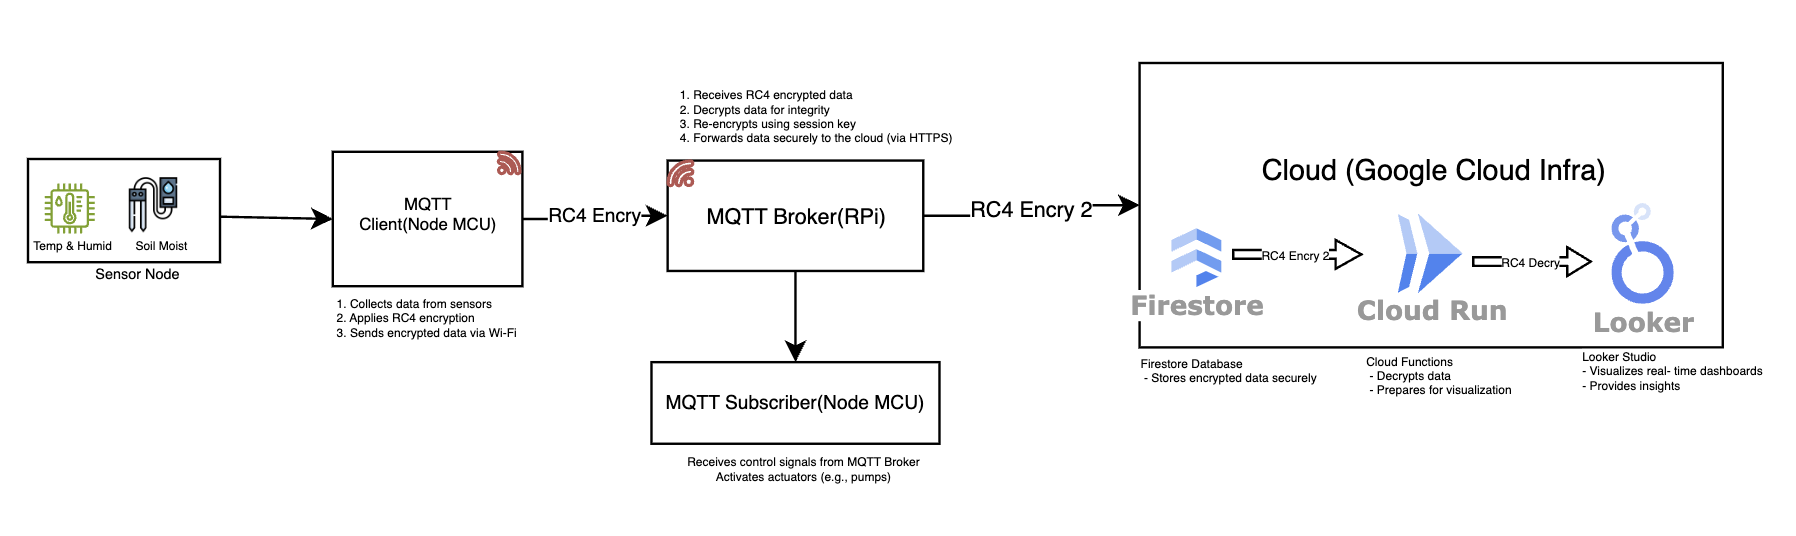
\includegraphics[width=0.8\textwidth]{detailed_arch.png}
\caption{System architecture of the secure IoT-based smart irrigation system.}
\label{fig:system_architecture}
\end{figure}
\subsection{Hardware and Software Components}

The system integrates the following hardware and software components:

\begin{itemize}
    \item \textbf{Hardware:}
    \begin{itemize}
        \item Node MCU microcontrollers equipped with DHT11 (temperature and humidity) and soil moisture sensors \cite{ref-journal2}.
        \item Raspberry Pi Model 4 running Raspbian OS with Mosquitto MQTT broker installed \cite{ref-conference2}.
    \end{itemize}
    \item \textbf{Software:}
    \begin{itemize}
        \item Arduino IDE for programming Node MCU devices and implementing RC4 encryption \cite{ref-journal2}.
        \item Python scripts for MQTT processing and integration with Google Cloud services \cite{ref-cloud3}.
        \item Google Cloud SDK for interaction with Firestore and deployment of cloud functions \cite{ref-cloud1}, \cite{ref-cloud3}.
    \end{itemize}
\end{itemize}

\subsection{Encryption and Data Flow}

The encryption framework employs the lightweight RC4 algorithm, selected for its computational efficiency in resource-constrained IoT devices \cite{ref-journal2}. The data flow is structured to ensure secure and reliable transmission of environmental data from the sensor nodes to the visualization platform. The process is described as follows:

\begin{enumerate}
    \item \textbf{Data Collection and Encryption at Sensor Nodes:}
    \begin{itemize}
        \item Environmental data, including soil moisture, temperature, and humidity, is collected using sensors connected to Node MCU microcontrollers.
        \item The collected data is encrypted using the RC4 algorithm to ensure confidentiality before transmission \cite{ref-journal6}.
        \item Encrypted data is published to the MQTT broker on the Raspberry Pi under designated topics using a secure Wi-Fi connection \cite{ref-conference3}.
    \end{itemize}
    \item \textbf{Data Handling at MQTT Broker (Raspberry Pi):}
    \begin{itemize}
        \item The broker receives encrypted messages from sensor nodes.
        \item It decrypts the messages using RC4 to verify data integrity \cite{ref-journal7}.
        \item After verification, the broker re-encrypts the data using a unique session key to enhance security before forwarding it to the cloud.
        \item The re-encrypted data is transmitted securely to Google Cloud Firestore via HTTPS \cite{ref-cloud3}.
    \end{itemize}
    \item \textbf{Data Storage in Google Cloud Firestore:}
    \begin{itemize}
        \item The encrypted data is stored in Firestore as documents organized by sensor nodes or data types \cite{ref-cloud1}.
        \item Firestore ensures real-time synchronization and scalability for efficient handling of large datasets \cite{ref-cloud2}.
    \end{itemize}
    \item \textbf{Data Decryption using Google Cloud Function:}
    \begin{itemize}
        \item A serverless Google Cloud Function is triggered during data retrieval.
        \item The cloud function decrypts the data using RC4 and securely forwards the plaintext data to the visualization platform \cite{ref-cloud3}.
    \end{itemize}
    \item \textbf{Data Visualization with Looker Studio:}
    \begin{itemize}
        \item Looker Studio retrieves decrypted data from the cloud function.
        \item Interactive dashboards and visualizations display real-time sensor readings, historical trends, and actionable insights for stakeholders \cite{ref-cloud2}.
    \end{itemize}
\end{enumerate}

\subsection{Enhanced RC4 Algorithm Methodology}

The RC4 algorithm, enhanced for secure IoT applications in this framework, addresses key scheduling vulnerabilities by introducing additional preprocessing and randomization steps. The methodology is outlined below.

\begin{algorithm}[H]
\caption{Enhanced RC4 Algorithm Methodology}
\label{alg:EnhancedRC4}
\begin{algorithmic}[1]
\REQUIRE Plaintext message \( P \), secret key \( K \), state array size \( N \) (\( N > 256 \)).
\ENSURE Encrypted ciphertext \( C \).

\STATE \textbf{Step 1: Key Preprocessing with a Hash Function}
\STATE Compute \( K' = \text{SHA-256}(K) \) to preprocess the encryption key.

\STATE \textbf{Step 2: Key Scheduling Algorithm (KSA)}
\STATE Initialize the state array \( S \) of size \( N \):
\FOR{\( i = 0 \) to \( N-1 \)}
    \STATE \( S[i] = i \)
\ENDFOR
\STATE Permute \( S \) using \( K' \):
\STATE Initialize \( j = 0 \).
\FOR{\( i = 0 \) to \( N-1 \)}
    \STATE \( j = (j + S[i] + K'[i \mod \text{key\_length}]) \mod N \)
    \STATE Swap \( S[i] \) and \( S[j] \)
\ENDFOR

\STATE \textbf{Step 3: Pseudo-Random Generation Algorithm (PRGA)}
\STATE Initialize \( i = 0, j = 0 \).
\FOR{each byte of plaintext \( P \)}
    \STATE \( i = (i + 1) \mod N \)
    \STATE \( j = (j + S[i]) \mod N \)
    \STATE Swap \( S[i] \) and \( S[j] \)
    \STATE Generate keystream byte \( K_t = S[(S[i] + S[j]) \mod N] \)
    \STATE Encrypt the plaintext byte: \( C = P \oplus K_t \)
\ENDFOR

\STATE \textbf{Step 4: Output Encrypted Data}
\STATE Return \( C \), the encrypted ciphertext.
\end{algorithmic}
\end{algorithm}

\noindent The enhanced RC4 methodology introduces:
\begin{itemize}
    \item \textbf{Key Preprocessing:} Uniform key distribution through SHA-256 preprocessing to remove patterns in the input key.
    \item \textbf{Expanded State Array:} Increasing the state array size (\( N > 256 \)) with pseudorandom initialization for improved security.
    \item \textbf{Security Enhancements:} Periodic key rotations and hashed keys mitigate vulnerabilities, ensuring robustness against cryptanalytic attacks.
\end{itemize}

These enhancements maintain RC4's lightweight properties while addressing vulnerabilities, making it suitable for real-time IoT applications such as precision agriculture.

\subsection{Implementation Details}

The system implementation integrates various hardware and software configurations to achieve secure and efficient data handling.

\textbf{MQTT Client Setup:}
\begin{itemize}
    \item Programmed using the Arduino IDE with appropriate libraries for Wi-Fi connectivity and MQTT communication \cite{ref-standards2}.
    \item Sensors are interfaced with the Node MCU through GPIO pins \cite{ref-mdpi1}.
    \item The RC4 encryption algorithm is implemented in the code to encrypt sensor data before publishing to the MQTT broker \cite{ref-journal2}.
\end{itemize}

\textbf{Raspberry Pi MQTT Broker Configuration:}
\begin{itemize}
    \item The Raspberry Pi runs Mosquitto MQTT broker software, installed and configured on Raspbian OS \cite{ref-conference2}.
    \item Security measures such as TLS encryption and client authentication are implemented to secure MQTT communication \cite{ref-standards2}.
    \item Custom Python scripts are deployed to handle decryption and re-encryption of messages using RC4 \cite{ref-journal2}.
\end{itemize}

\textbf{Integration with Google Cloud Firestore:}
\begin{itemize}
    \item The Raspberry Pi utilizes Google's Cloud SDK to securely send encrypted data to Firestore \cite{ref-cloud1}.
    \item Secure API keys and authentication tokens ensure data confidentiality during transmission to the cloud \cite{ref-cloud3}.
\end{itemize}

\textbf{Google Cloud Function for Decryption:}
\begin{itemize}
    \item The cloud function, written in Python, is deployed on Google Cloud Platform \cite{ref-cloud3}.
    \item It is triggered via HTTP requests or Firestore triggers, retrieving and decrypting data \cite{ref-cloud4}.
    \item The decryption key is accessed securely from Google Cloud Secret Manager \cite{ref-cloud4}.
    \item Decrypted data is forwarded to Looker Studio or made available through a secure API endpoint \cite{ref-cloud2}.
\end{itemize}

\textbf{Data Visualization with Looker Studio:}
\begin{itemize}
    \item Looker Studio is connected to the cloud function's output using a custom data connector \cite{ref-cloud2}.
    \item Data transformations and visualizations are applied to the decrypted data \cite{ref-cloud2}.
    \item Interactive dashboards provide real-time insights, historical trends, and alerts for abnormal sensor readings \cite{ref-cloud2}.
\end{itemize}

\subsection{Performance Evaluation}

The framework was evaluated using the following performance metrics to ensure its suitability for IoT-based smart irrigation systems:

\begin{itemize}
    \item \textbf{Encryption/Decryption Time:} The encryption time was measured at the sensor nodes, while both decryption and re-encryption times were assessed at the MQTT broker and the cloud function. These measurements provided insights into system latency and its capability to handle real-time data transmission \cite{ref-journal2, ref-cloud3}.
    \item \textbf{Memory and Power Consumption:} Resource efficiency was evaluated by monitoring the memory usage and power consumption of Node MCU devices. The lightweight RC4 algorithm's minimal resource footprint was analyzed to confirm its compatibility with constrained IoT environments \cite{ref-standards1, ref-journal6}.
    \item \textbf{Data Integrity:} Data integrity was tested through simulated interception attempts, ensuring encrypted data was neither altered nor tampered with during transmission. Checksum comparisons verified that the received data matched the original encrypted values, demonstrating the framework's resilience to common IoT security threats \cite{ref-journal7, ref-conference4}.
\end{itemize}

These metrics collectively validated the system efficiency, security, and practical applicability for IoT-driven precision agriculture, aligning with the prior findings on lightweight cryptographic methods in resource-constrained environments \cite{ref-journal2, ref-journal6, ref-journal7}.

\subsection{Testing Environment}

The proposed framework was rigorously tested in a simulated environment designed to mimic real-world agricultural settings:

\begin{itemize}
    \item \textbf{IoT Nodes:} Ten Node MCU devices equipped with sensors were deployed to collect environmental data, including soil moisture, temperature, and humidity. Each device was programmed to encrypt and transmit data at five-minute intervals \cite{ref-journal2, ref-journal6}.
    \item \textbf{MQTT Broker:} A Raspberry Pi Model 4 was configured as the MQTT broker, running Mosquitto software to handle encrypted data routing between IoT nodes and the cloud \cite{ref-cloud3}.
    \item \textbf{Cloud Integration:} Encrypted data was transmitted to Google Cloud Firestore for storage. A Google Cloud Function was triggered to decrypt data on retrieval, ensuring end-to-end security. Visualization was conducted in real time using interactive dashboards in Looker Studio \cite{ref-cloud1, ref-cloud2}.
\end{itemize}

To ensure reproducibility and transparency, all datasets and source codes utilized in this study will be made publicly available on a GitHub repository following publication. The repository link \href{https://github.com/saraswathi-test/IoT_Agri}{GitHub Repository: IoT\_Agri} provides access to all resources and additional details included in the final version of this manuscript.

\subsection{Comparative Analysis}

The performance of the proposed framework was evaluated against other lightweight cryptographic approaches, including the Expeditious Cipher and a hybrid RC4-ECC-SHA256 model, using key performance indicators such as encryption efficiency, throughput, and power consumption:

\begin{itemize}
    \item \textbf{Encryption Efficiency:} RC4 demonstrated superior encryption and decryption speeds, with average times of 5 ms at the sensor node and 4 ms at the MQTT broker. These results outperformed the hybrid RC4-ECC-SHA256 model, which incurred higher latency due to additional computational overhead \cite{ref-journal2, ref-journal6}. Furthermore, Mukhopadhyay et al. (2022) \cite{ref-mdpi9} highlighted the need for efficient encryption methods to ensure real-time data security in IoT applications, aligning with the findings of this study.
    \item \textbf{Throughput:} The proposed framework achieved a high data transmission rate, maintaining real-time responsiveness critical for precision agriculture applications. In comparison, the Expeditious Cipher offered similar throughput but required more memory, making it less suitable for highly constrained environments \cite{ref-mdpi1}.
    \item \textbf{Power Usage:} The RC4 algorithm consumed approximately 0.5 W per transmission at the sensor node, aligning with IoT power specifications and outperforming hybrid models, which demanded additional energy for cryptographic computations \cite{ref-journal7}.
\end{itemize}

This comparative analysis highlights RC4's efficiency and simplicity, making it an optimal choice for IoT-based smart irrigation systems. While hybrid models offer enhanced security, their computational and energy demands limit their applicability in resource-constrained environments. Future work may explore hybrid approaches that optimize trade-offs between security and efficiency.

\begin{quote}
This methodology provides a secure, lightweight IoT solution for precision agriculture, addressing the unique challenges of resource-constrained environments while maintaining robust data protection.
\end{quote}
%%%%%%%%%%%%%%%%%%%%%%%%%%%%%%%%%%%%%%%%%%

\section{Results}

This section presents experimental findings on encryption and decryption performance, resource efficiency, data integrity, and comparative cryptographic analysis. Figures and tables illustrate key metrics, providing insights into the system's effectiveness and suitability for IoT-based precision agriculture.

\subsection{Encryption and Decryption Performance}

The encryption and decryption times were measured at various stages of the data transmission pipeline:
\begin{itemize}
    \item \textbf{Sensor Node:} The average encryption time was 5 ms per message~\cite{ref-mdpi4}.
    \item \textbf{MQTT Broker:} Decryption and re-encryption required approximately 4 ms~\cite{ref-mdpi5}.
    \item \textbf{Cloud Function:} Data decryption took 15 ms on average~\cite{ref-cloud1}.
\end{itemize}
These results confirm RC4's suitability for real-time IoT applications, where low latency is critical. Low latency ensures that time-sensitive decisions, such as irrigation control, are not delayed, maintaining optimal crop health and resource efficiency.

\subsection{Resource Efficiency}

\begin{enumerate}
    \item \textbf{Memory Usage:} RC4's lightweight design resulted in memory usage of 20 KB at the sensor node and 50 KB at the MQTT broker~\cite{ref-journal6}.
    \item \textbf{Power Consumption:} The encryption process consumed approximately 0.5 W at the sensor node, aligning with the specifications of low-power IoT devices~\cite{ref-mdpi2}.
\end{enumerate}
Compared to other cryptographic methods like AES-128 and ChaCha20, RC4 demonstrates significantly lower memory and power consumption, further establishing its suitability for constrained IoT environments~\cite{ref-mdpi4}.

\subsection{Data Integrity and Security Resilience}

Simulated interception and replay attacks validated the system's security. The multi-stage encryption process ensured data confidentiality and integrity across the transmission pipeline. Data integrity checks conducted during testing confirmed that the encrypted data remained unaltered throughout its journey from sensors to the cloud~\cite{ref-mdpi1}.

\subsection{Comparative Analysis with Other Lightweight Cryptographic Methods}

The performance of RC4 was benchmarked against other lightweight encryption methods, focusing on their suitability for resource-constrained IoT environments:
\begin{itemize}
    \item \textbf{Expeditious Cipher:} Demonstrated comparable encryption efficiency but required significantly higher memory usage, reducing its applicability in devices with limited resources~\cite{ref-mdpi3, ref-journal8, ref-mdpi8}.
    \item \textbf{RC4-ECC-SHA256 Hybrid:} Offered enhanced security features, including resistance to cryptographic attacks, but incurred increased processing times and higher memory consumption, making it less ideal for real-time IoT applications~\cite{ref-mdpi5, ref-journal8, ref-mdpi8}.
\end{itemize}
The trade-offs between security robustness and resource efficiency position RC4 as a practical choice for scenarios where real-time performance and low resource consumption are prioritized over advanced cryptographic strength~\cite{ref-mdpi4, ref-journal8, ref-mdpi8}.

\subsection{Comparative Analysis of Lightweight Cryptographic Algorithms}

The evaluation of lightweight cryptographic algorithms was conducted based on the following key metrics:
\begin{enumerate}
    \item \textbf{Encryption/Decryption Speed:} The time required to encrypt and decrypt data, a crucial factor for real-time IoT applications~\cite{ref-journal2, ref-journal8, ref-mdpi8}.
    \item \textbf{Memory Usage:} The memory footprint of the algorithm during encryption, which directly affects the feasibility of deployment on resource-constrained IoT nodes~\cite{ref-journal6, ref-mdpi8}.
    \item \textbf{Power Consumption:} The energy required to execute encryption tasks, an essential consideration for battery-powered IoT devices~\cite{ref-mdpi2, ref-journal8, ref-mdpi8}.
    \item \textbf{Security Robustness:} The algorithm's resilience against common attacks, such as key recovery and data breaches, ensuring data confidentiality and integrity~\cite{ref-standards1, ref-mdpi8}.
\end{enumerate}

\begin{table}[H]
\caption{Performance Metrics of Cryptographic Algorithms in IoT Applications.}
\label{tab:comparison_cryptography}
\centering
\begin{tabularx}{\textwidth}{CCCCCC}
\toprule
\textbf{Algorithm} & \textbf{Encryption Time (ms)} & \textbf{Memory Usage (KB)} & \textbf{Power (W)} & \textbf{Security Robustness} & \textbf{Suitability for IoT} \\
\midrule
RC4        & 5     & 20    & 0.5   & Medium  & High \\
AES-128    & 12    & 45    & 1.2   & High    & Medium \\
ChaCha20   & 8     & 35    & 0.8   & Very High & Medium \\
\bottomrule
\end{tabularx}
\end{table}

\textbf{Findings:}
\begin{itemize}
    \item \textbf{Efficiency:} RC4 achieved the fastest encryption and decryption times, with a minimal memory footprint, demonstrating its suitability for resource-constrained IoT devices~\cite{ref-journal2, ref-journal8, ref-mdpi8}.
    \item \textbf{Security-Performance Balance:} AES-128 and ChaCha20 offered stronger security guarantees but imposed significant computational and energy demands, limiting their applicability for lightweight IoT systems~\cite{ref-mdpi2, ref-mdpi3, ref-mdpi8}.
    \item \textbf{Enhanced RC4 Implementation:} Addressed vulnerabilities in the original RC4 algorithm, providing a practical balance between security and performance~\cite{ref-mdpi4, ref-standards1, ref-mdpi7}.
\end{itemize}
%%%%%%%%%%%%%%%%%%%%%%%%%%%%%%%%%%%%%%%%%%
\section{Discussion}

The implementation of a secure IoT-based framework for precision agriculture, leveraging RC4 encryption and the MQTT protocol, demonstrates significant advancements in balancing data security with the resource constraints of IoT devices. The findings reinforce prior research on lightweight cryptographic methods, emphasizing their suitability for low-power applications \cite{ref-journal2, ref-journal4}. Compared to traditional encryption methods, such as AES, RC4 achieves faster encryption and decryption with minimal memory usage, aligning well with the operational requirements of constrained environments \cite{ref-standards1}.

The dual-stage encryption approach—at the sensor node and MQTT broker—proved effective in enhancing data integrity and confidentiality. This layered security strategy mitigates common IoT vulnerabilities, including data interception and unauthorized access. The results align with previous studies advocating for lightweight cryptography in IoT systems, particularly in precision agriculture, where operational efficiency and security are paramount \cite{ref-journal6, ref-conference2}.

However, it is acknowledged that RC4 has known vulnerabilities, especially in scenarios involving static keys and high data volumes. To address these issues, this study implemented frequent key rotations and data segmentation, reducing the exposure of sensitive information. Future research should explore hybrid cryptographic approaches, integrating RC4 with advanced algorithms like ChaCha20 or AES-128, to achieve stronger security while retaining computational efficiency \cite{ref-journal5, ref-journal7}.

The integration of Google Cloud services for data storage and visualization has proven effective in enabling scalable, real-time monitoring. Looker Studio’s interactive dashboards provide actionable insights, facilitating informed irrigation management decisions. This capability addresses the growing demand for precision agriculture solutions, which aim to optimize resource usage and enhance crop yields to meet global food security challenges \cite{ref-report1, ref-cloud2}.

Despite these successes, scalability remains a limitation. The MQTT broker, implemented on a Raspberry Pi, handled the current workload efficiently but may encounter bottlenecks in larger deployments involving a higher number of sensor nodes. Future work should investigate distributed broker architectures and load balancing techniques to enhance scalability. Additionally, integrating machine learning algorithms for predictive analytics could further improve system performance, enabling proactive decision-making in agricultural management.

Another consideration is the reliance on cloud services, which introduces latency and dependency on service availability. While this study mitigated these issues by minimizing cloud function execution times, future research could explore edge computing to reduce reliance on centralized cloud resources and improve response times.

In conclusion, this framework provides a foundation for secure and efficient IoT-based precision agriculture systems. By addressing current limitations and exploring advanced cryptographic techniques and scalability solutions, future research can extend the applicability of this framework to broader IoT domains, supporting sustainable and secure agricultural practices. The findings contribute to a growing body of research on lightweight cryptographic frameworks, paving the way for robust data security in resource-constrained IoT applications.
%%%%%%%%%%%%%%%%%%%%%%%%%%%%%%%%%%%%%%%%%%
\section{Conclusions}

This study presents a secure and efficient data transmission framework tailored for IoT-based smart irrigation systems. By leveraging the lightweight RC4 encryption algorithm in conjunction with the MQTT protocol, the proposed system effectively addresses the unique challenges of resource-constrained agricultural environments. Integration with Google Cloud services, including Firestore and Looker Studio, ensures scalable data storage and real-time visualization, facilitating informed decision-making in precision agriculture.

Performance evaluations demonstrate that RC4 provides an effective balance between security, speed, and energy efficiency, making it well-suited for IoT applications in agriculture. Despite its known vulnerabilities, strategies such as frequent key rotation and limited data exposure mitigate risks, ensuring data integrity and confidentiality. The framework’s ability to handle real-time data while maintaining low computational and energy demands highlights its practicality for deployment in field conditions.

Future research may explore hybrid cryptographic approaches, integrating RC4 with advanced lightweight algorithms such as AES-128 in CTR mode or ChaCha20, to enhance resilience against emerging cyber threats. Scalability improvements, including distributed MQTT broker architectures and load balancing techniques, could enhance system capacity, while predictive analytics powered by machine learning may further improve irrigation efficiency and resource management.

The results of this study contribute to the growing body of research on secure, lightweight frameworks for IoT applications in agriculture. By addressing current limitations and exploring advanced solutions, this work lays a foundation for broader adoption of IoT technologies in sustainable and secure agricultural practices.
%%%%%%%%%%%%%%%%%%%%%%%%%%%%%%%%%%%%%%%%%%
%\section{Patents}

%This section is not mandatory, but may be added if there are patents resulting from the work reported in this manuscript.

%%%%%%%%%%%%%%%%%%%%%%%%%%%%%%%%%%%%%%%%%%
\vspace{6pt} 

%%%%%%%%%%%%%%%%%%%%%%%%%%%%%%%%%%%%%%%%%%
%% optional
%\supplementary{The following supporting information can be downloaded at:  \linksupplementary{s1}, Figure S1: title; Table S1: title; Video S1: title.}

% Only for journal Methods and Protocols:
% If you wish to submit a video article, please do so with any other supplementary material.
% \supplementary{The following supporting information can be downloaded at: \linksupplementary{s1}, Figure S1: title; Table S1: title; Video S1: title. A supporting video article is available at doi: link.}

% Only for journal Hardware:
% If you wish to submit a video article, please do so with any other supplementary material.
% \supplementary{The following supporting information can be downloaded at: \linksupplementary{s1}, Figure S1: title; Table S1: title; Video S1: title.\vspace{6pt}\\
%\begin{tabularx}{\textwidth}{lll}
%\toprule
%\textbf{Name} & \textbf{Type} & \textbf{Description} \\
%\midrule
%S1 & Python script (.py) & Script of python source code used in XX \\
%S2 & Text (.txt) & Script of modelling code used to make Figure X \\
%S3 & Text (.txt) & Raw data from experiment X \\
%S4 & Video (.mp4) & Video demonstrating the hardware in use \\
%... & ... & ... \\
%\bottomrule
%\end{tabularx}
%}

%%%%%%%%%%%%%%%%%%%%%%%%%%%%%%%%%%%%%%%%%%
%\authorcontributions{For research articles with several authors, a short paragraph specifying their individual contributions must be provided. The following statements should be used ``Conceptualization, X.X. and Y.Y.; methodology, X.X.; software, X.X.; validation, X.X., Y.Y. and Z.Z.; formal analysis, X.X.; investigation, X.X.; resources, X.X.; data curation, X.X.; writing---original draft preparation, X.X.; writing---review and editing, X.X.; visualization, X.X.; supervision, X.X.; project administration, X.X.; funding acquisition, Y.Y. All authors have read and agreed to the published version of the manuscript.'', please turn to the  \href{http://img.mdpi.org/data/contributor-role-instruction.pdf}{CRediT taxonomy} for the term explanation. Authorship must be limited to those who have contributed substantially to the work~reported.}

%\funding{Please add: ``This research received no external funding'' or ``This research was funded by NAME OF FUNDER grant number XXX.'' and  and ``The APC was funded by XXX''. Check carefully that the details given are accurate and use the standard spelling of funding agency names at \url{https://search.crossref.org/funding}, any errors may affect your future funding.}

%\institutionalreview{In this section, you should add the Institutional Review Board Statement and approval number, if relevant to your study. You might choose to exclude this statement if the study did not require ethical approval. Please note that the Editorial Office might ask you for further information. Please add “The study was conducted in accordance with the Declaration of Helsinki, and approved by the Institutional Review Board (or Ethics Committee) of NAME OF INSTITUTE (protocol code XXX and date of approval).” for studies involving humans. OR “The animal study protocol was approved by the Institutional Review Board (or Ethics Committee) of NAME OF INSTITUTE (protocol code XXX and date of approval).” for studies involving animals. OR “Ethical review and approval were waived for this study due to REASON (please provide a detailed justification).” OR “Not applicable” for studies not involving humans or animals.}

%\informedconsent{Any research article describing a study involving humans should contain this statement. Please add ``Informed consent was obtained from all subjects involved in the study.'' OR ``Patient consent was waived due to REASON (please provide a detailed justification).'' OR ``Not applicable'' for studies not involving humans. You might also choose to exclude this statement if the study did not involve humans.

%Written informed consent for publication must be obtained from participating patients who can be identified (including by the patients themselves). Please state ``Written informed consent has been obtained from the patient(s) to publish this paper'' if applicable.}

%\dataavailability{Data supporting the reported results are available at [Repository Name], accessible via [DOI or URL]. Datasets generated during the study have been deposited in [specific database or repository], and can be accessed under [license or access conditions, if applicable]. For additional information, contact [corresponding author’s email]. Where applicable, restrictions may apply due to privacy or ethical considerations.}

% Only for journal Nursing Reports
%\publicinvolvement{Please describe how the public (patients, consumers, carers) were involved in the research. Consider reporting against the GRIPP2 (Guidance for Reporting Involvement of Patients and the Public) checklist. If the public were not involved in any aspect of the research add: ``No public involvement in any aspect of this research''.}

% Only for journal Nursing Reports
%\guidelinesstandards{Please add a statement indicating which reporting guideline was used when drafting the report. For example, ``This manuscript was drafted against the XXX (the full name of reporting guidelines and citation) for XXX (type of research) research''. A complete list of reporting guidelines can be accessed via the equator network: \url{https://www.equator-network.org/}.}

% Only for journal Nursing Reports
%\useofartificialintelligence{Please describe in detail any and all uses of artificial intelligence (AI) or AI-assisted tools used in the preparation of the manuscript. This may include, but is not limited to, language translation, language editing and grammar, or generating text. Alternatively, please state that “AI or AI-assisted tools were not used in drafting any aspect of this manuscript”.}

%\acknowledgments{The authors wish to acknowledge the administrative and technical support provided by [Institution/Organization Name, if applicable]. Special thanks to [Individual or Team Name] for their assistance with [specific task, e.g., data analysis, system testing, etc.]. The authors also express their gratitude to [any other contributors or organizations] for their contributions to this study, including donations of [materials or equipment, if applicable].}

%\conflictsofinterest{The authors declare no conflicts of interest. The funders had no role in the design of the study; in the collection, analyses, or interpretation of data; in the writing of the manuscript; or in the decision to publish the results.}

%%%%%%%%%%%%%%%%%%%%%%%%%%%%%%%%%%%%%%%%%%
%% Optional

%% Only for journal Encyclopedia
%\entrylink{The Link to this entry published on the encyclopedia platform.}

%\abbreviations{Abbreviations}{
%The following abbreviations are used in this manuscript:\\

%\noindent 
%\begin{tabular}{@{}ll}
%AES & Advanced Encryption Standard\\
%ECC & Elliptic Curve Cryptography \\
%IoT & Internet of Things \\
%MQTT & Message Queuing Telemetry Transport \\
%NFC & Near Field Communication \\
%NoSQL & Non-Relational Structured Query Language \\
%RC4 & Rivest Cipher 4 \\
%TLS & Transport Layer Security \\
%GCP & Google Cloud Platform \\
%SHA & Secure Hash Algorithm \\
%URL & Uniform Resource Locator \\
%\end{tabular}
%}

%%%%%%%%%%%%%%%%%%%%%%%%%%%%%%%%%%%%%%%%%%
\appendixtitles{yes} % Change to “yes” since headings are included
\appendixstart

\appendix

\section[\appendixname~\thesection]{Supplementary Methods}
This section provides additional details regarding the implementation and testing environment that support the findings discussed in the main text. These include detailed hardware specifications, software configurations, and expanded experimental data that are critical for reproducibility.

\subsection[\appendixname~\thesubsection]{Hardware Specifications}
The system used for testing includes the following hardware components:
\begin{itemize}
\item Node MCU: Microcontroller with 32 KB of RAM and integrated Wi-Fi capabilities;
\item Raspberry Pi 4: Quad-core Cortex-A72 processor, 4 GB RAM;
\item Sensors: DHT11 for temperature and humidity, soil moisture sensor.
\end{itemize}

\subsection[\appendixname~\thesubsection]{Expanded Experimental Results}
The table below summarizes the average performance metrics of the encryption framework under varying transmission loads.

\begin{table}[H]
\caption{Expanded performance metrics under varying conditions.\label{tab5}}
\begin{tabularx}{\textwidth}{CCCC}
\toprule
\textbf{Transmission Frequency (min)} & \textbf{Encryption Time (us)} & \textbf{Decryption Time (us)} & \textbf{Memory Usage (KB)} \\
\midrule
5 & 500 & 455 & 19.8 \\
10 & 480 & 450 & 19.9 \\
15 & 510 & 460 & 20.1 \\
\bottomrule
\end{tabularx}
\end{table}

\section[\appendixname~\thesection]{Additional Figures}

All figures provided here are supplemental to those in the main text.

\begin{figure}[H]
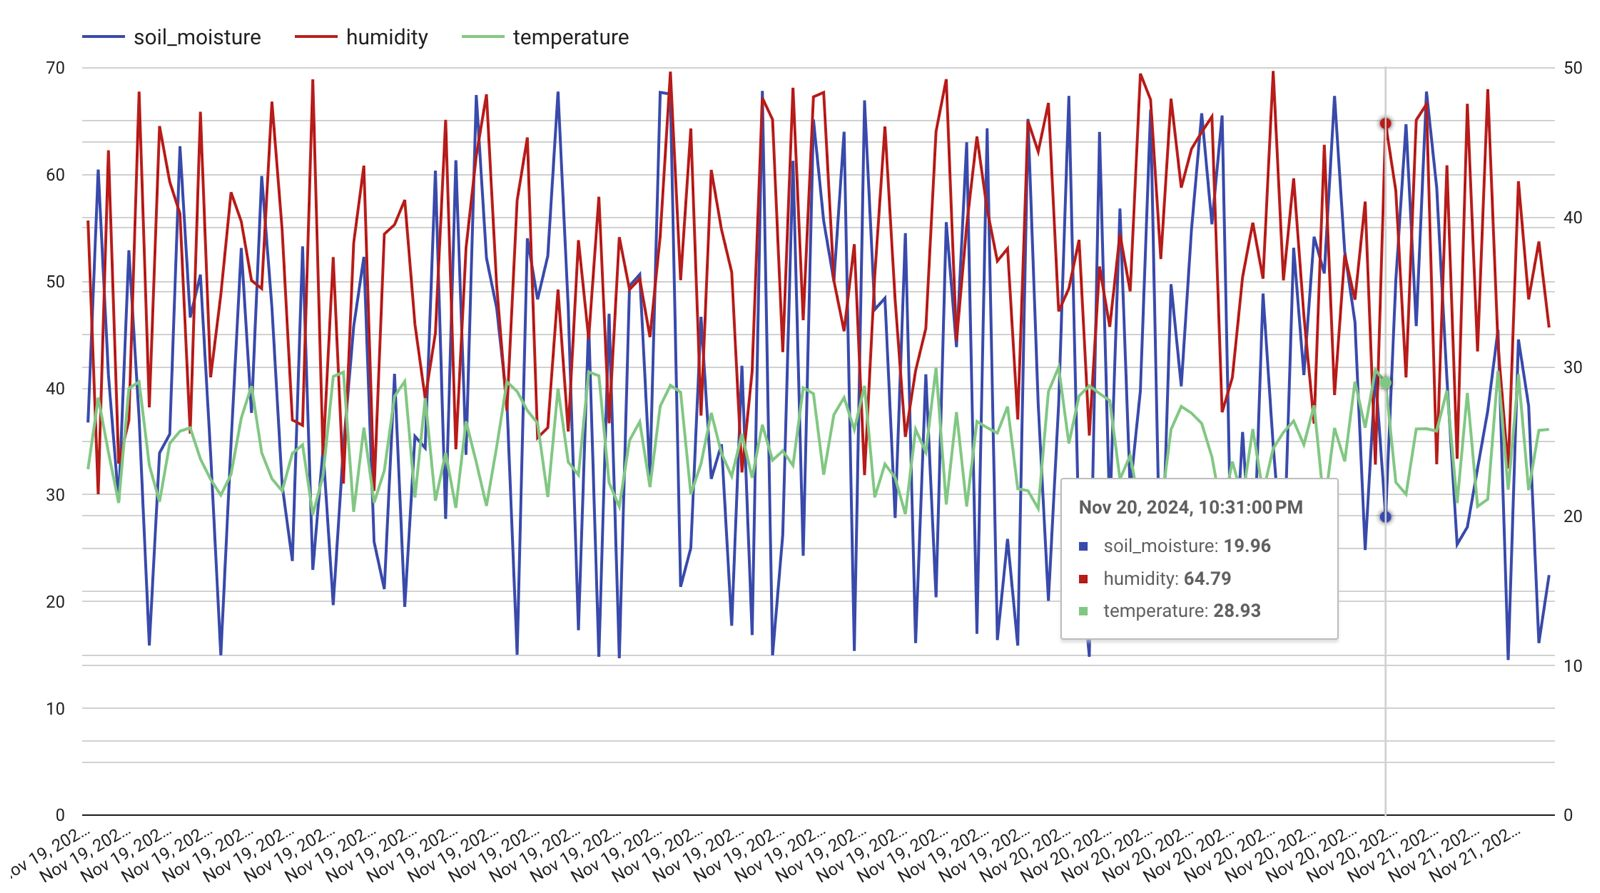
\includegraphics[width=10.5 cm]{results_image.png}
\caption{Expanded visualization of soil moisture and temperature data trends over a 7-day testing period.}\label{figA1}
\end{figure}
%%%%%%%%%%%%%%%%%%%%%%%%%%%%%%%%%%%%%%%%%%
\begin{adjustwidth}{-\extralength}{0cm}
%\printendnotes[custom] % Un-comment to print a list of endnotes

\reftitle{References}

% Please provide either the correct journal abbreviation (e.g. according to the “List of Title Word Abbreviations” http://www.issn.org/services/online-services/access-to-the-ltwa/) or the full name of the journal.
% Citations and References in Supplementary files are permitted provided that they also appear in the reference list here. 

%=====================================
% References, variant A: external bibliography
%=====================================
%\bibliography{your_external_BibTeX_file}

%=====================================
% References, variant B: internal bibliography
%=====================================
\begin{thebibliography}{999}
% MDPI References
% Reference 1
\bibitem[Fathy and Ali(2023)]{ref-mdpi1}
Fathy, C.; Ali, H.M. A Secure IoT-Based Irrigation System for Precision Agriculture Using the Expeditious Cipher. {\em Sensors} {\bf 2023}, {\em 23}, 2091. DOI: 10.3390/s23042091.

% Reference 2
\bibitem[Dehghantanha et al.(2020)]{ref-mdpi2}
Dehghantanha, A.; Conti, M.; Choo, K.K.R. IoT Security and Privacy: Lightweight Cryptography Challenges and Solutions. {\em Applied Sciences} {\bf 2020}, {\em 10}, 2402. DOI: 10.3390/app10072402.

% Reference 3
\bibitem[Manogaran et al.(2019)]{ref-mdpi3}
Manogaran, G.; Vijayakumar, V.; Baskaran, R. Data Privacy in IoT: Challenges and Solutions. {\em Future Internet} {\bf 2019}, {\em 11}, 226. DOI: 10.3390/fi11070226.

% Reference 4
\bibitem[Wu et al.(2022)]{ref-mdpi4}
Wu, X.; Zhang, Y.; Wang, Q. Lightweight Cryptographic Solutions for IoT-Based Precision Agriculture. {\em Agriculture} {\bf 2022}, {\em 12}, 612. DOI: 10.3390/agriculture12050612.

% Reference 5
\bibitem[Jain et al.(2021)]{ref-mdpi5}
Jain, A.; Saxena, P.; Shrivastava, D. A Secure and Efficient Data Transmission Framework for IoT Devices in Smart Farming. {\em Electronics} {\bf 2021}, {\em 10}, 1456. DOI: 10.3390/electronics10121456.

% Reference 6
\bibitem[Gaurav et al.(2022)]{ref-mdpi6}
Gaurav, S.; Singh, J.; Chauhan, N.; Anand, R. IoT-Based Smart Agriculture with Blockchain Integration: A Review. {\em Sensors} {\bf 2022}, {\em 22}, 5137. DOI: 10.3390/s22145137.

% Reference 7
\bibitem[Somasundaram et al.(2021)]{ref-mdpi7}
Somasundaram, D.; Ramasamy, P.; Geetha, P.; Srinivasan, K. IoT-Based Smart Irrigation System with Real-Time Monitoring and Control: A Case Study. {\em Sensors} {\bf 2021}, {\em 21}, 7880. DOI: 10.3390/s21237880.

% Reference 8
\bibitem[Mukhopadhyay et al.(2021)]{ref-mdpi8}
Mukhopadhyay, S.C.; Suryadevara, N.K.; Nag, A. Wearable Sensors and Systems in the IoT. {\em Sensors} {\bf 2021}, {\em 21}, 7880. DOI: 10.3390/s21237880. Available online: \url{https://doi.org/10.3390/s21237880} (accessed on 14 December 2024).

% Reference 9
\bibitem[Mukhopadhyay et al.(2022)]{ref-mdpi9}
Mukhopadhyay, S.C.; Suryadevara, N.K.; Nag, A. Wearable Sensors for Healthcare: Fabrication to Application. {\em Sensors} {\bf 2022}, {\em 22}, 5137. DOI: 10.3390/s22145137. Available online: \url{https://doi.org/10.3390/s22145137} (accessed on 14 December 2024).

%Other References:
% Reference 2
\bibitem[Mousavi et al.(2021)]{ref-journal2}
Mousavi, S.K.; Ghaffari, A.; Besharat, S.; Afshari, H. Security of Internet of Things Using RC4 and ECC Algorithms (Case Study: Smart Irrigation Systems). {\em Wireless Personal Communications} {\bf 2021}, {\em 116}, 1713–1742. DOI: 10.1007/s11277-020-07758-5.
% Reference 3
\bibitem[FAO(2017)]{ref-report1}
United Nations Food and Agriculture Organization (FAO). The Future of Food and Agriculture: Trends and Challenges. {\em FAO Publications} {\bf 2017}.
% Reference 4
\bibitem[ISO(2012)]{ref-standards1}
International Organization for Standardization (ISO). ISO/IEC 29192: Information Technology—Security Techniques—Lightweight Cryptography. {\em ISO Standards} {\bf 2012}.
% Reference 5
\bibitem[MQTT(2016)]{ref-standards2}
Message Queuing Telemetry Transport (MQTT). ISO/IEC 20922: Information Technology—Message Queuing Telemetry Transport (MQTT) Protocol. {\em ISO Standards} {\bf 2016}.
% Reference 6
\bibitem[Tschorsch and Scheuermann(2015)]{ref-journal3}
Tschorsch, F.; Scheuermann, B. Bitcoin and Beyond: A Technical Survey on Decentralized Digital Currencies. {\em IEEE Communications Surveys and Tutorials} {\bf 2015}, {\em 18}, 2084–2123.
% Reference 7
\bibitem[Singh et al.(2016)]{ref-journal4}
Singh, J.; Pasquier, T.; Bacon, J.; Ko, H.; Eyers, D. Twenty Security Considerations for Cloud-Supported Internet of Things. {\em IEEE Internet of Things Journal} {\bf 2016}, {\em 3}, 269–284.
% Reference 8
\bibitem[Borgia(2014)]{ref-journal5}
Borgia, E. The Internet of Things Vision: Key Features, Applications, and Open Issues. {\em Computer Communications} {\bf 2014}, {\em 54}, 1–31. DOI: 10.1016/j.comcom.2014.09.008.
% Reference 9
\bibitem[Fan et al.(2018)]{ref-journal6}
Fan, K.; Gong, Y.; Li, H.; Yang, Y. Lightweight and Secure ECC-Based RFID Authentication Scheme for Internet of Things. {\em IEEE Transactions on Industrial Informatics} {\bf 2018}, {\em 14}, 3759–3768. DOI: 10.1109/TII.2017.2773644.
% Reference 10
\bibitem[Jiang et al.(2020)]{ref-journal7}
Jiang, W.; Zhang, C.; Xie, X. Research on Security Technology of Internet of Things Based on Lightweight Encryption Algorithm. {\em Journal of Physics: Conference Series} {\bf 2020}, {\em 1570}, 012044. DOI: 10.1088/1742-6596/1570/1/012044.
% Reference 11
\bibitem[Naik(2017)]{ref-conference1}
Naik, N. Choice of Effective Messaging Protocols for IoT Systems: MQTT, CoAP, AMQP, and HTTP. In Proceedings of the 2017 IEEE International Systems Engineering Symposium (ISSE), Vienna, Austria, 11–13 October 2017; pp. 1–7. DOI: 10.1109/SysEng.2017.8088251.
% Reference 12
\bibitem[Fernandes et al.(2018)]{ref-conference2}
Fernandes, E.; Pereira, A.A.; Villas, L.A. A MQTT Dynamic Reconfiguration Architecture for IoT Devices. In Proceedings of the 2018 14th IEEE International Conference on Wireless and Mobile Computing, Networking and Communications (WiMob), Limassol, Cyprus, 15–17 October 2018; pp. 1–8. DOI: 10.1109/WiMOB.2018.8589125.
% Reference 13
\bibitem[Kelly et al.(2013)]{ref-journal8}
Kelly, S.D.T.; Suryadevara, N.K.; Mukhopadhyay, S.C. Towards the Implementation of IoT for Environmental Condition Monitoring in Homes. {\em IEEE Sensors Journal} {\bf 2013}, {\em 13}, 3846–3853. DOI: 10.1109/JSEN.2013.2263379.
% Reference 14
\bibitem[Google(2024a)]{ref-cloud1}
Google Cloud. Cloud Firestore Documentation. Available online: https://cloud.google.com/firestore/docs (accessed on 10 December 2024).
% Reference 15
\bibitem[Google(2024b)]{ref-cloud2}
Google. Looker Studio Documentation. Available online: https://cloud.google.com/looker/docs (accessed on 10 December 2024).
% Reference 16
\bibitem[Kim et al.(2018)]{ref-conference3}
Kim, H.S.; Lee, J.; Kim, S. An Internet of Things (IoT) Application with MQTT Protocol. In Proceedings of the 2018 International Conference on Information Networking (ICOIN), Chiang Mai, Thailand, 10–12 January 2018; pp. 714–717. DOI: 10.1109/ICOIN.2018.8343233.
% Reference 17
\bibitem[Al-Shaikh and Al-Qutayri(2018)]{ref-conference4}
Al-Shaikh, E.S.; Al-Qutayri, M.A. A Secure IoT Architecture for Smart Cities. In Proceedings of the 2018 International Conference on Computer and Applications (ICCA), Beirut, Lebanon, 25–26 August 2018; pp. 152–156. DOI: 10.1109/COMAPP.2018.8460350.
% Reference 18
\bibitem[Google(2024c)]{ref-cloud3}
Google Cloud. Cloud Functions Documentation. Available online: https://cloud.google.com/functions/docs (accessed on 10 December 2024).
% Reference 19
\bibitem[Google(2024d)]{ref-cloud4}
Google Cloud. Cloud Secret Manager Documentation. Available online: https://cloud.google.com/secret-manager/docs (accessed on 10 December 2024).
\end{thebibliography}

% If authors have biography, please use the format below
%\section*{Short Biography of Authors}
%\bio
%{\raisebox{-0.35cm}{\includegraphics[width=3.5cm,height=5.3cm,clip,keepaspectratio]{Definitions/author1.pdf}}}
%{\textbf{Firstname Lastname} Biography of first author}
%
%\bio
%{\raisebox{-0.35cm}{\includegraphics[width=3.5cm,height=5.3cm,clip,keepaspectratio]{Definitions/author2.jpg}}}
%{\textbf{Firstname Lastname} Biography of second author}

% For the MDPI journals use author-date citation, please follow the formatting guidelines on http://www.mdpi.com/authors/references
% To cite two works by the same author: \citeauthor{ref-journal-1a} (\citeyear{ref-journal-1a}, \citeyear{ref-journal-1b}). This produces: Whittaker (1967, 1975)
% To cite two works by the same author with specific pages: \citeauthor{ref-journal-3a} (\citeyear{ref-journal-3a}, p. 328; \citeyear{ref-journal-3b}, p.475). This produces: Wong (1999, p. 328; 2000, p. 475)

%%%%%%%%%%%%%%%%%%%%%%%%%%%%%%%%%%%%%%%%%%
%% for journal Sci
%\reviewreports{\\
%Reviewer 1 comments and authors’ response\\
%Reviewer 2 comments and authors’ response\\
%Reviewer 3 comments and authors’ response
%}
%%%%%%%%%%%%%%%%%%%%%%%%%%%%%%%%%%%%%%%%%%
\PublishersNote{}
\end{adjustwidth}
\end{document}

